\section{Navegação} % (fold)
\label{sec:navegação2}
	
	Como o processamento de todas as informações obtidas durante a navegação ocorrerá na base, sabe-se que o tempo de resposta do servidor é uma variável importante quando se refere a um sistema de tempo real, como o proposto pelo projeto. Dessa maneira, fez-se necessária a implantação do \textit{patch} \textit{rt\_preempt} no kernel do linux presente na \textit{raspberry}. Para isso, utilizamos como fonte de conhecimento a wiki oficial do projeto \textit{RT\_preempt}, disponível \href{https://rt.wiki.kernel.org/index.php/Main_Page}{aqui}.

	Com a configuração e recompilação do kernel com este \textit{patch}, obtivemos um tempo de resposta aproximado de 19 micro segundos, o que foi considerado bom pela equipe do projeto. Uma análise foi feita utilizando o \textit{script} \textit{cylicltest}, da mesma equipe \textit{RT\_preempt}, para calcular o tempo mínimo, médio e máximo de resposta. Na simulação foi utilizado um processo com prioridade 80, com 100.000 (cem mil) \textit{loops} a um intervalo de 500 micro segundos, obtendo o resultado apresentado na Figura \ref{img:tempo_de_resposta}.

	\begin{figure}[H]
		\centering
		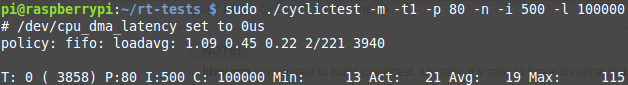
\includegraphics[scale=0.7]{figuras/tempo_de_resposta.png}
		\caption{Tempo de resposta do servidor.}
		\label{img:tempo_de_resposta}
	\end{figure}

% section navegação (end)